\documentclass[1p]{elsarticle_modified}
%\bibliographystyle{elsarticle-num}

%\usepackage[colorlinks]{hyperref}
%\usepackage{abbrmath_seonhwa} %\Abb, \Ascr, \Acal ,\Abf, \Afrak
\usepackage{amsfonts}
\usepackage{amssymb}
\usepackage{amsmath}
\usepackage{amsthm}
\usepackage{scalefnt}
\usepackage{amsbsy}
\usepackage{kotex}
\usepackage{caption}
\usepackage{subfig}
\usepackage{color}
\usepackage{graphicx}
\usepackage{xcolor} %% white, black, red, green, blue, cyan, magenta, yellow
\usepackage{float}
\usepackage{setspace}
\usepackage{hyperref}

\usepackage{tikz}
\usetikzlibrary{arrows}

\usepackage{multirow}
\usepackage{array} % fixed length table
\usepackage{hhline}

%%%%%%%%%%%%%%%%%%%%%
\makeatletter
\renewcommand*\env@matrix[1][\arraystretch]{%
	\edef\arraystretch{#1}%
	\hskip -\arraycolsep
	\let\@ifnextchar\new@ifnextchar
	\array{*\c@MaxMatrixCols c}}
\makeatother %https://tex.stackexchange.com/questions/14071/how-can-i-increase-the-line-spacing-in-a-matrix
%%%%%%%%%%%%%%%

\usepackage[normalem]{ulem}

\newcommand{\msout}[1]{\ifmmode\text{\sout{\ensuremath{#1}}}\else\sout{#1}\fi}
%SOURCE: \msout is \stkout macro in https://tex.stackexchange.com/questions/20609/strikeout-in-math-mode

\newcommand{\cancel}[1]{
	\ifmmode
	{\color{red}\msout{#1}}
	\else
	{\color{red}\sout{#1}}
	\fi
}

\newcommand{\add}[1]{
	{\color{blue}\uwave{#1}}
}

\newcommand{\replace}[2]{
	\ifmmode
	{\color{red}\msout{#1}}{\color{blue}\uwave{#2}}
	\else
	{\color{red}\sout{#1}}{\color{blue}\uwave{#2}}
	\fi
}

\newcommand{\Sol}{\mathcal{S}} %segment
\newcommand{\D}{D} %diagram
\newcommand{\A}{\mathcal{A}} %arc


%%%%%%%%%%%%%%%%%%%%%%%%%%%%%5 test

\def\sl{\operatorname{\textup{SL}}(2,\Cbb)}
\def\psl{\operatorname{\textup{PSL}}(2,\Cbb)}
\def\quan{\mkern 1mu \triangleright \mkern 1mu}

\theoremstyle{definition}
\newtheorem{thm}{Theorem}[section]
\newtheorem{prop}[thm]{Proposition}
\newtheorem{lem}[thm]{Lemma}
\newtheorem{ques}[thm]{Question}
\newtheorem{cor}[thm]{Corollary}
\newtheorem{defn}[thm]{Definition}
\newtheorem{exam}[thm]{Example}
\newtheorem{rmk}[thm]{Remark}
\newtheorem{alg}[thm]{Algorithm}

\newcommand{\I}{\sqrt{-1}}
\begin{document}

%\begin{frontmatter}
%
%\title{Boundary parabolic representations of knots up to 8 crossings}
%
%%% Group authors per affiliation:
%\author{Yunhi Cho} 
%\address{Department of Mathematics, University of Seoul, Seoul, Korea}
%\ead{yhcho@uos.ac.kr}
%
%
%\author{Seonhwa Kim} %\fnref{s_kim}}
%\address{Center for Geometry and Physics, Institute for Basic Science, Pohang, 37673, Korea}
%\ead{ryeona17@ibs.re.kr}
%
%\author{Hyuk Kim}
%\address{Department of Mathematical Sciences, Seoul National University, Seoul 08826, Korea}
%\ead{hyukkim@snu.ac.kr}
%
%\author{Seokbeom Yoon}
%\address{Department of Mathematical Sciences, Seoul National University, Seoul, 08826,  Korea}
%\ead{sbyoon15@snu.ac.kr}
%
%\begin{abstract}
%We find all boundary parabolic representation of knots up to 8 crossings.
%
%\end{abstract}
%\begin{keyword}
%    \MSC[2010] 57M25 
%\end{keyword}
%
%\end{frontmatter}

%\linenumbers
%\tableofcontents
%
\newcommand\colored[1]{\textcolor{white}{\rule[-0.35ex]{0.8em}{1.4ex}}\kern-0.8em\color{red} #1}%
%\newcommand\colored[1]{\textcolor{white}{ #1}\kern-2.17ex	\textcolor{white}{ #1}\kern-1.81ex	\textcolor{white}{ #1}\kern-2.15ex\color{red}#1	}

{\Large $\underline{12n_{0680}~(K12n_{0680})}$}

\setlength{\tabcolsep}{10pt}
\renewcommand{\arraystretch}{1.6}
\vspace{1cm}\begin{tabular}{m{100pt}>{\centering\arraybackslash}m{274pt}}
\multirow{5}{120pt}{
	\centering
	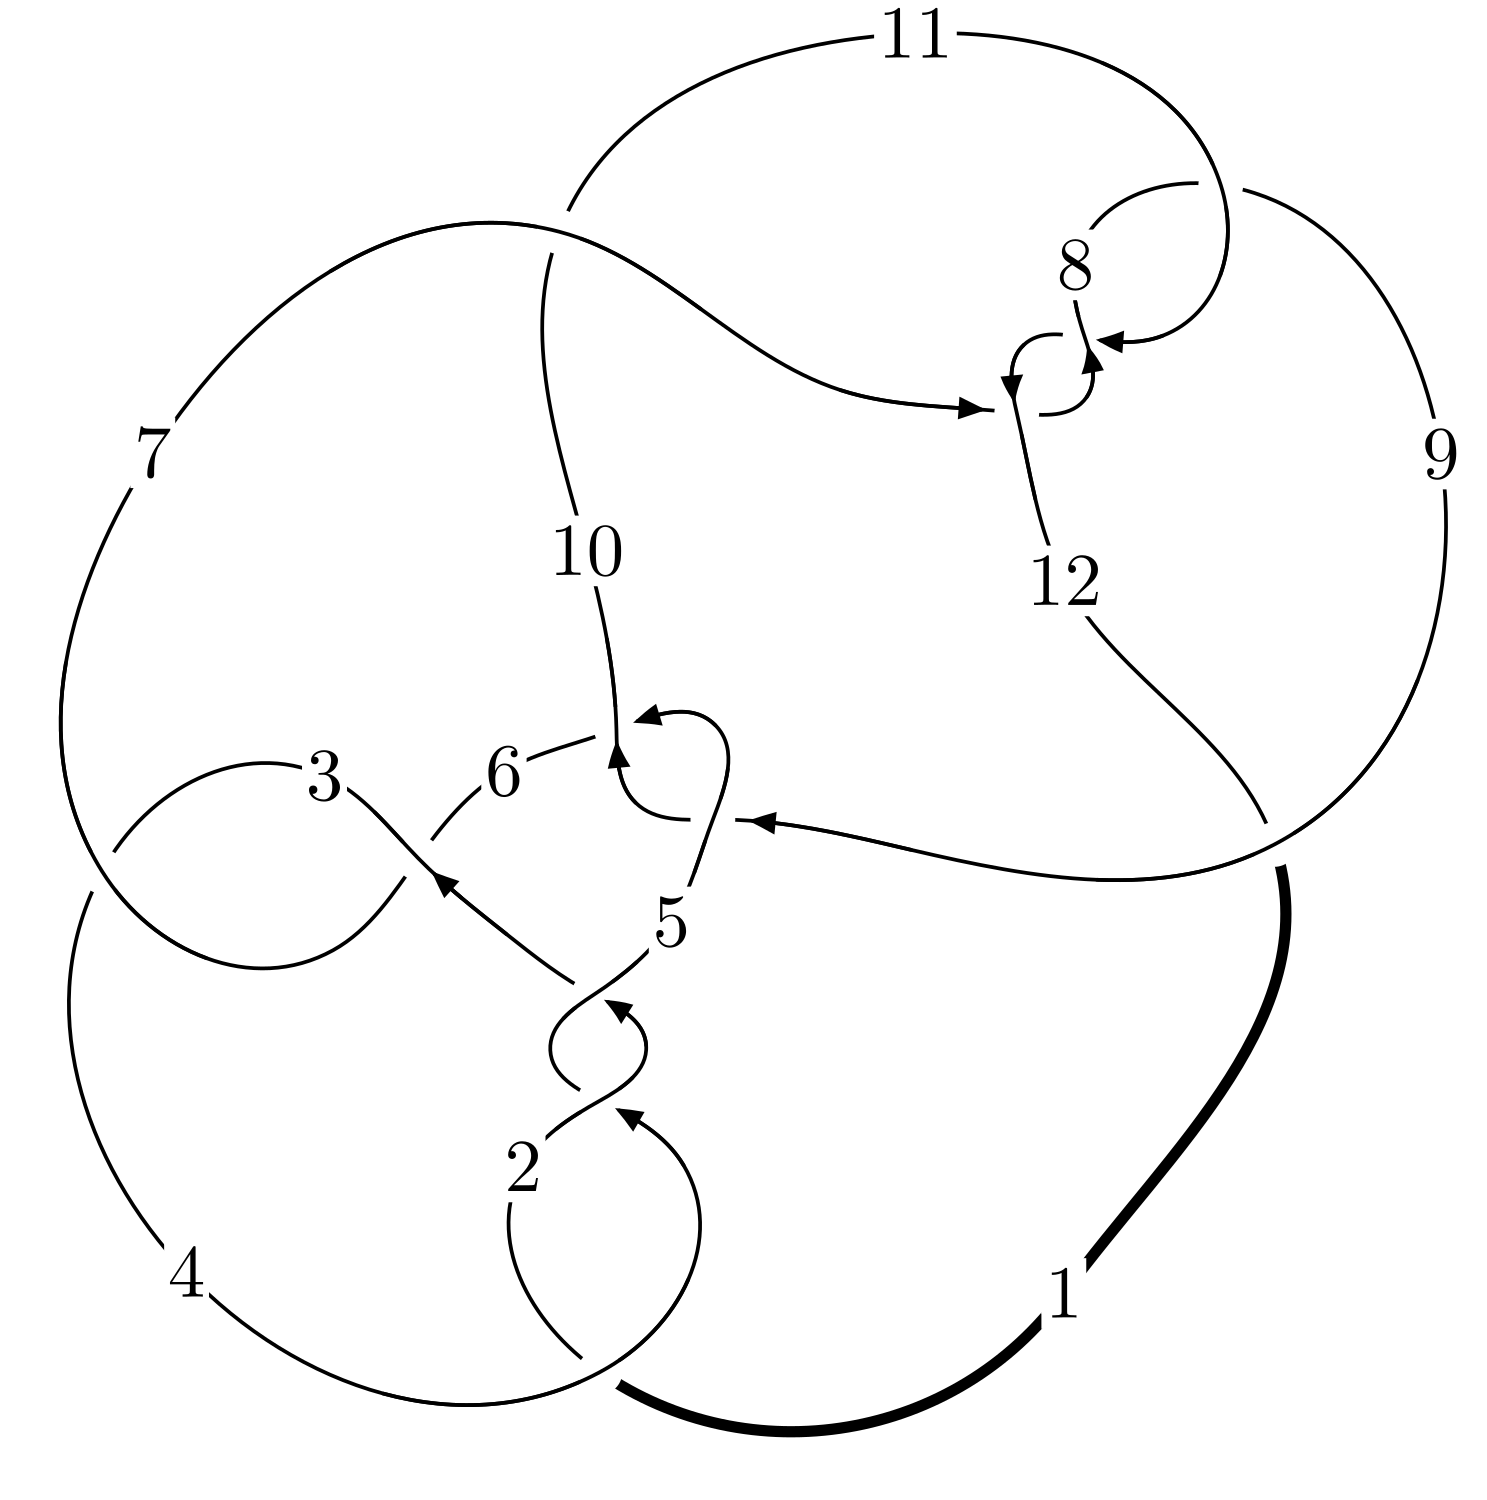
\includegraphics[width=112pt]{../../../GIT/diagram.site/Diagrams/png/2769_12n_0680.png}\\
\ \ \ A knot diagram\footnotemark}&
\allowdisplaybreaks
\textbf{Linearized knot diagam} \\
\cline{2-2}
 &
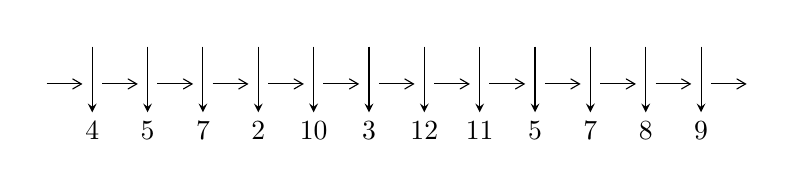
\begin{tikzpicture}[x=20pt, y=17pt]
	% nodes
	\node (C0) at (0, 0) {};
	\node (C1) at (1, 0) {};
	\node (C1U) at (1, +1) {};
	\node (C1D) at (1, -1) {4};

	\node (C2) at (2, 0) {};
	\node (C2U) at (2, +1) {};
	\node (C2D) at (2, -1) {5};

	\node (C3) at (3, 0) {};
	\node (C3U) at (3, +1) {};
	\node (C3D) at (3, -1) {7};

	\node (C4) at (4, 0) {};
	\node (C4U) at (4, +1) {};
	\node (C4D) at (4, -1) {2};

	\node (C5) at (5, 0) {};
	\node (C5U) at (5, +1) {};
	\node (C5D) at (5, -1) {10};

	\node (C6) at (6, 0) {};
	\node (C6U) at (6, +1) {};
	\node (C6D) at (6, -1) {3};

	\node (C7) at (7, 0) {};
	\node (C7U) at (7, +1) {};
	\node (C7D) at (7, -1) {12};

	\node (C8) at (8, 0) {};
	\node (C8U) at (8, +1) {};
	\node (C8D) at (8, -1) {11};

	\node (C9) at (9, 0) {};
	\node (C9U) at (9, +1) {};
	\node (C9D) at (9, -1) {5};

	\node (C10) at (10, 0) {};
	\node (C10U) at (10, +1) {};
	\node (C10D) at (10, -1) {7};

	\node (C11) at (11, 0) {};
	\node (C11U) at (11, +1) {};
	\node (C11D) at (11, -1) {8};

	\node (C12) at (12, 0) {};
	\node (C12U) at (12, +1) {};
	\node (C12D) at (12, -1) {9};
	\node (C13) at (13, 0) {};

	% arrows
	\draw[->,>={angle 60}]
	(C0) edge (C1) (C1) edge (C2) (C2) edge (C3) (C3) edge (C4) (C4) edge (C5) (C5) edge (C6) (C6) edge (C7) (C7) edge (C8) (C8) edge (C9) (C9) edge (C10) (C10) edge (C11) (C11) edge (C12) (C12) edge (C13) ;	\draw[->,>=stealth]
	(C1U) edge (C1D) (C2U) edge (C2D) (C3U) edge (C3D) (C4U) edge (C4D) (C5U) edge (C5D) (C6U) edge (C6D) (C7U) edge (C7D) (C8U) edge (C8D) (C9U) edge (C9D) (C10U) edge (C10D) (C11U) edge (C11D) (C12U) edge (C12D) ;
	\end{tikzpicture} \\
\hhline{~~} \\& 
\textbf{Solving Sequence} \\ \cline{2-2} 
 &
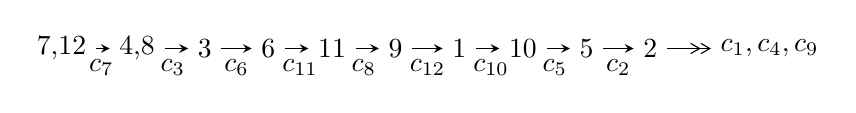
\begin{tikzpicture}[x=23pt, y=7pt]
	% node
	\node (A0) at (-1/8, 0) {7,12};
	\node (A1) at (17/16, 0) {4,8};
	\node (A2) at (17/8, 0) {3};
	\node (A3) at (25/8, 0) {6};
	\node (A4) at (33/8, 0) {11};
	\node (A5) at (41/8, 0) {9};
	\node (A6) at (49/8, 0) {1};
	\node (A7) at (57/8, 0) {10};
	\node (A8) at (65/8, 0) {5};
	\node (A9) at (73/8, 0) {2};
	\node (C1) at (1/2, -1) {$c_{7}$};
	\node (C2) at (13/8, -1) {$c_{3}$};
	\node (C3) at (21/8, -1) {$c_{6}$};
	\node (C4) at (29/8, -1) {$c_{11}$};
	\node (C5) at (37/8, -1) {$c_{8}$};
	\node (C6) at (45/8, -1) {$c_{12}$};
	\node (C7) at (53/8, -1) {$c_{10}$};
	\node (C8) at (61/8, -1) {$c_{5}$};
	\node (C9) at (69/8, -1) {$c_{2}$};
	\node (A10) at (11, 0) {$c_{1},c_{4},c_{9}$};

	% edge
	\draw[->,>=stealth]	
	(A0) edge (A1) (A1) edge (A2) (A2) edge (A3) (A3) edge (A4) (A4) edge (A5) (A5) edge (A6) (A6) edge (A7) (A7) edge (A8) (A8) edge (A9) ;
	\draw[->>,>={angle 60}]	
	(A9) edge (A10);
\end{tikzpicture} \\ 

\end{tabular} \\

\footnotetext{
The image of knot diagram is generated by the software ``\textbf{Draw programme}" developed by Andrew Bartholomew(\url{http://www.layer8.co.uk/maths/draw/index.htm\#Running-draw}), where we modified some parts for our purpose(\url{https://github.com/CATsTAILs/LinksPainter}).
}\phantom \\ \newline 
\centering \textbf{Ideals for irreducible components\footnotemark of $X_{\text{par}}$} 
 
\begin{align*}
I^u_{1}&=\langle 
3449 u^{20}+3669 u^{19}+\cdots+71498 b-42457,\;-23077 u^{20}-82531 u^{19}+\cdots+71498 a+43556,\\
\phantom{I^u_{1}}&\phantom{= \langle  }u^{21}+4 u^{20}+\cdots-2 u+1\rangle \\
I^u_{2}&=\langle 
b,\;u^5+2 u^4+4 u^3+4 u^2+a+3 u+2,\;u^6+u^5+3 u^4+2 u^3+2 u^2+u-1\rangle \\
I^u_{3}&=\langle 
- a u+b- u,\;- u^2 a+a^2+a u-3 u^2+2 u-4,\;u^3- u^2+2 u-1\rangle \\
\\
\end{align*}
\raggedright * 3 irreducible components of $\dim_{\mathbb{C}}=0$, with total 33 representations.\\
\footnotetext{All coefficients of polynomials are rational numbers. But the coefficients are sometimes approximated in decimal forms when there is not enough margin.}
\newpage
\renewcommand{\arraystretch}{1}
\centering \section*{I. $I^u_{1}= \langle 3449 u^{20}+3669 u^{19}+\cdots+71498 b-42457,\;-23077 u^{20}-82531 u^{19}+\cdots+71498 a+43556,\;u^{21}+4 u^{20}+\cdots-2 u+1 \rangle$}
\flushleft \textbf{(i) Arc colorings}\\
\begin{tabular}{m{7pt} m{180pt} m{7pt} m{180pt} }
\flushright $a_{7}=$&$\begin{pmatrix}1\\0\end{pmatrix}$ \\
\flushright $a_{12}=$&$\begin{pmatrix}0\\u\end{pmatrix}$ \\
\flushright $a_{4}=$&$\begin{pmatrix}0.322764 u^{20}+1.15431 u^{19}+\cdots+4.24348 u-0.609192\\-0.0482391 u^{20}-0.0513161 u^{19}+\cdots-0.0347422 u+0.593821\end{pmatrix}$ \\
\flushright $a_{8}=$&$\begin{pmatrix}1\\u^2\end{pmatrix}$ \\
\flushright $a_{3}=$&$\begin{pmatrix}0.274525 u^{20}+1.10300 u^{19}+\cdots+4.20873 u-0.0153711\\-0.0482391 u^{20}-0.0513161 u^{19}+\cdots-0.0347422 u+0.593821\end{pmatrix}$ \\
\flushright $a_{6}=$&$\begin{pmatrix}-0.224552 u^{20}-1.13479 u^{19}+\cdots-2.45920 u+0.935718\\0.166117 u^{20}+0.596254 u^{19}+\cdots+0.165739 u-0.324387\end{pmatrix}$ \\
\flushright $a_{11}=$&$\begin{pmatrix}u\\u^3+u\end{pmatrix}$ \\
\flushright $a_{9}=$&$\begin{pmatrix}u^2+1\\u^4+2 u^2\end{pmatrix}$ \\
\flushright $a_{1}=$&$\begin{pmatrix}- u^5-2 u^3- u\\- u^7-3 u^5-2 u^3+u\end{pmatrix}$ \\
\flushright $a_{10}=$&$\begin{pmatrix}u^3+2 u\\u^3+u\end{pmatrix}$ \\
\flushright $a_{5}=$&$\begin{pmatrix}-0.406179 u^{20}-1.57648 u^{19}+\cdots-2.97737 u+0.847101\\-0.0482391 u^{20}-0.0513161 u^{19}+\cdots-0.0347422 u-0.406179\end{pmatrix}$ \\
\flushright $a_{2}=$&$\begin{pmatrix}0.0868835 u^{20}+0.255951 u^{19}+\cdots+1.16347 u+0.290428\\0.0482391 u^{20}+0.0513161 u^{19}+\cdots+0.0347422 u+0.406179\end{pmatrix}$\\&\end{tabular}
\flushleft \textbf{(ii) Obstruction class $= -1$}\\~\\
\flushleft \textbf{(iii) Cusp Shapes $= -\frac{58626}{35749} u^{20}-\frac{459843}{71498} u^{19}+\cdots+\frac{105825}{71498} u-\frac{777975}{71498}$}\\~\\
\newpage\renewcommand{\arraystretch}{1}
\flushleft \textbf{(iv) u-Polynomials at the component}\newline \\
\begin{tabular}{m{50pt}|m{274pt}}
Crossings & \hspace{64pt}u-Polynomials at each crossing \\
\hline $$\begin{aligned}c_{1},c_{2},c_{4}\end{aligned}$$&$\begin{aligned}
&u^{21}-10 u^{20}+\cdots-4 u-1
\end{aligned}$\\
\hline $$\begin{aligned}c_{3},c_{6}\end{aligned}$$&$\begin{aligned}
&u^{21}+4 u^{20}+\cdots-128 u+64
\end{aligned}$\\
\hline $$\begin{aligned}c_{5},c_{9}\end{aligned}$$&$\begin{aligned}
&u^{21}-2 u^{20}+\cdots+224 u+64
\end{aligned}$\\
\hline $$\begin{aligned}c_{7},c_{8},c_{11}\end{aligned}$$&$\begin{aligned}
&u^{21}-4 u^{20}+\cdots-2 u-1
\end{aligned}$\\
\hline $$\begin{aligned}c_{10},c_{12}\end{aligned}$$&$\begin{aligned}
&u^{21}+4 u^{20}+\cdots-304 u-97
\end{aligned}$\\
\hline
\end{tabular}\\~\\
\newpage\renewcommand{\arraystretch}{1}
\flushleft \textbf{(v) Riley Polynomials at the component}\newline \\
\begin{tabular}{m{50pt}|m{274pt}}
Crossings & \hspace{64pt}Riley Polynomials at each crossing \\
\hline $$\begin{aligned}c_{1},c_{2},c_{4}\end{aligned}$$&$\begin{aligned}
&y^{21}-4 y^{20}+\cdots+152 y-1
\end{aligned}$\\
\hline $$\begin{aligned}c_{3},c_{6}\end{aligned}$$&$\begin{aligned}
&y^{21}+30 y^{20}+\cdots+90112 y-4096
\end{aligned}$\\
\hline $$\begin{aligned}c_{5},c_{9}\end{aligned}$$&$\begin{aligned}
&y^{21}+28 y^{20}+\cdots+82944 y-4096
\end{aligned}$\\
\hline $$\begin{aligned}c_{7},c_{8},c_{11}\end{aligned}$$&$\begin{aligned}
&y^{21}+22 y^{20}+\cdots-10 y-1
\end{aligned}$\\
\hline $$\begin{aligned}c_{10},c_{12}\end{aligned}$$&$\begin{aligned}
&y^{21}+14 y^{20}+\cdots-131266 y-9409
\end{aligned}$\\
\hline
\end{tabular}\\~\\
\newpage\flushleft \textbf{(vi) Complex Volumes and Cusp Shapes}
$$\begin{array}{c|c|c}  
\text{Solutions to }I^u_{1}& \I (\text{vol} + \sqrt{-1}CS) & \text{Cusp shape}\\
 \hline 
\begin{aligned}
u &= -0.904622 + 0.417722 I \\
a &= \phantom{-}1.45274 - 0.01148 I \\
b &= \phantom{-}0.92182 - 2.09929 I\end{aligned}
 & \phantom{-}6.05963 + 7.34750 I & -14.4555 - 4.2838 I \\ \hline\begin{aligned}
u &= -0.904622 - 0.417722 I \\
a &= \phantom{-}1.45274 + 0.01148 I \\
b &= \phantom{-}0.92182 + 2.09929 I\end{aligned}
 & \phantom{-}6.05963 - 7.34750 I & -14.4555 + 4.2838 I \\ \hline\begin{aligned}
u &= -0.766571 + 0.752408 I \\
a &= -1.037380 + 0.144450 I \\
b &= \phantom{-}0.29405 + 2.35369 I\end{aligned}
 & \phantom{-}7.09375 - 1.76941 I & -12.87851 - 0.26190 I \\ \hline\begin{aligned}
u &= -0.766571 - 0.752408 I \\
a &= -1.037380 - 0.144450 I \\
b &= \phantom{-}0.29405 - 2.35369 I\end{aligned}
 & \phantom{-}7.09375 + 1.76941 I & -12.87851 + 0.26190 I \\ \hline\begin{aligned}
u &= \phantom{-}0.182461 + 1.208850 I \\
a &= -0.276557 - 0.201585 I \\
b &= -0.119527 + 0.423528 I\end{aligned}
 & \phantom{-}2.74625 - 2.07596 I & -5.86030 + 3.17371 I \\ \hline\begin{aligned}
u &= \phantom{-}0.182461 - 1.208850 I \\
a &= -0.276557 + 0.201585 I \\
b &= -0.119527 - 0.423528 I\end{aligned}
 & \phantom{-}2.74625 + 2.07596 I & -5.86030 - 3.17371 I \\ \hline\begin{aligned}
u &= -0.734798\phantom{ +0.000000I} \\
a &= -1.01042\phantom{ +0.000000I} \\
b &= -1.32151\phantom{ +0.000000I}\end{aligned}
 & -10.5256\phantom{ +0.000000I} & -25.3380\phantom{ +0.000000I} \\ \hline\begin{aligned}
u &= \phantom{-}0.200947 + 1.339400 I \\
a &= -1.31937 + 2.00455 I \\
b &= -0.552581 - 0.279603 I\end{aligned}
 & \phantom{-}1.78822 - 2.54403 I & -24.8123 + 5.5170 I \\ \hline\begin{aligned}
u &= \phantom{-}0.200947 - 1.339400 I \\
a &= -1.31937 - 2.00455 I \\
b &= -0.552581 + 0.279603 I\end{aligned}
 & \phantom{-}1.78822 + 2.54403 I & -24.8123 - 5.5170 I \\ \hline\begin{aligned}
u &= -0.341638 + 1.336290 I \\
a &= \phantom{-}0.828590 - 0.644391 I \\
b &= -1.256020 - 0.461833 I\end{aligned}
 & -6.25683 + 3.88389 I & -16.6815 - 2.9719 I\\
 \hline 
 \end{array}$$\newpage$$\begin{array}{c|c|c}  
\text{Solutions to }I^u_{1}& \I (\text{vol} + \sqrt{-1}CS) & \text{Cusp shape}\\
 \hline 
\begin{aligned}
u &= -0.341638 - 1.336290 I \\
a &= \phantom{-}0.828590 + 0.644391 I \\
b &= -1.256020 + 0.461833 I\end{aligned}
 & -6.25683 - 3.88389 I & -16.6815 + 2.9719 I \\ \hline\begin{aligned}
u &= \phantom{-}0.512237\phantom{ +0.000000I} \\
a &= -5.60059\phantom{ +0.000000I} \\
b &= -0.289328\phantom{ +0.000000I}\end{aligned}
 & -2.52473\phantom{ +0.000000I} & -76.9450\phantom{ +0.000000I} \\ \hline\begin{aligned}
u &= -0.35905 + 1.50519 I \\
a &= \phantom{-}0.78634 + 2.07126 I \\
b &= \phantom{-}1.39494 - 1.98909 I\end{aligned}
 & \phantom{-}12.2217 + 11.9532 I & -11.90704 - 5.00504 I \\ \hline\begin{aligned}
u &= -0.35905 - 1.50519 I \\
a &= \phantom{-}0.78634 - 2.07126 I \\
b &= \phantom{-}1.39494 + 1.98909 I\end{aligned}
 & \phantom{-}12.2217 - 11.9532 I & -11.90704 + 5.00504 I \\ \hline\begin{aligned}
u &= \phantom{-}0.06735 + 1.55292 I \\
a &= -1.37220 + 0.85690 I \\
b &= \phantom{-}1.86679 - 0.98776 I\end{aligned}
 & \phantom{-}5.79361 - 0.73866 I & -10.20116 + 0.28003 I \\ \hline\begin{aligned}
u &= \phantom{-}0.06735 - 1.55292 I \\
a &= -1.37220 - 0.85690 I \\
b &= \phantom{-}1.86679 + 0.98776 I\end{aligned}
 & \phantom{-}5.79361 + 0.73866 I & -10.20116 - 0.28003 I \\ \hline\begin{aligned}
u &= -0.21280 + 1.64374 I \\
a &= -0.63755 - 2.25205 I \\
b &= -0.62112 + 3.12830 I\end{aligned}
 & \phantom{-}15.1889 + 1.8962 I & -10.30157 - 0.70895 I \\ \hline\begin{aligned}
u &= -0.21280 - 1.64374 I \\
a &= -0.63755 + 2.25205 I \\
b &= -0.62112 - 3.12830 I\end{aligned}
 & \phantom{-}15.1889 - 1.8962 I & -10.30157 + 0.70895 I \\ \hline\begin{aligned}
u &= \phantom{-}0.334401\phantom{ +0.000000I} \\
a &= -0.860564\phantom{ +0.000000I} \\
b &= \phantom{-}0.297521\phantom{ +0.000000I}\end{aligned}
 & -0.669543\phantom{ +0.000000I} & -14.6190\phantom{ +0.000000I} \\ \hline\begin{aligned}
u &= \phantom{-}0.077997 + 0.278544 I \\
a &= -0.18883 + 1.76255 I \\
b &= \phantom{-}0.728300 - 0.059767 I\end{aligned}
 & -0.764279 + 0.134030 I & -11.95123 + 0.33972 I\\
 \hline 
 \end{array}$$\newpage$$\begin{array}{c|c|c}  
\text{Solutions to }I^u_{1}& \I (\text{vol} + \sqrt{-1}CS) & \text{Cusp shape}\\
 \hline 
\begin{aligned}
u &= \phantom{-}0.077997 - 0.278544 I \\
a &= -0.18883 - 1.76255 I \\
b &= \phantom{-}0.728300 + 0.059767 I\end{aligned}
 & -0.764279 - 0.134030 I & -11.95123 - 0.33972 I\\
 \hline 
 \end{array}$$\newpage\newpage\renewcommand{\arraystretch}{1}
\centering \section*{II. $I^u_{2}= \langle b,\;u^5+2 u^4+4 u^3+4 u^2+a+3 u+2,\;u^6+u^5+3 u^4+2 u^3+2 u^2+u-1 \rangle$}
\flushleft \textbf{(i) Arc colorings}\\
\begin{tabular}{m{7pt} m{180pt} m{7pt} m{180pt} }
\flushright $a_{7}=$&$\begin{pmatrix}1\\0\end{pmatrix}$ \\
\flushright $a_{12}=$&$\begin{pmatrix}0\\u\end{pmatrix}$ \\
\flushright $a_{4}=$&$\begin{pmatrix}- u^5-2 u^4-4 u^3-4 u^2-3 u-2\\0\end{pmatrix}$ \\
\flushright $a_{8}=$&$\begin{pmatrix}1\\u^2\end{pmatrix}$ \\
\flushright $a_{3}=$&$\begin{pmatrix}- u^5-2 u^4-4 u^3-4 u^2-3 u-2\\0\end{pmatrix}$ \\
\flushright $a_{6}=$&$\begin{pmatrix}1\\0\end{pmatrix}$ \\
\flushright $a_{11}=$&$\begin{pmatrix}u\\u^3+u\end{pmatrix}$ \\
\flushright $a_{9}=$&$\begin{pmatrix}u^2+1\\u^4+2 u^2\end{pmatrix}$ \\
\flushright $a_{1}=$&$\begin{pmatrix}- u^5-2 u^3- u\\- u^5- u^4-2 u^3- u^2- u+1\end{pmatrix}$ \\
\flushright $a_{10}=$&$\begin{pmatrix}u^3+2 u\\u^3+u\end{pmatrix}$ \\
\flushright $a_{5}=$&$\begin{pmatrix}u^5+2 u^3+u\\u^5+u^4+2 u^3+u^2+u-1\end{pmatrix}$ \\
\flushright $a_{2}=$&$\begin{pmatrix}-2 u^5-2 u^4-6 u^3-4 u^2-4 u-2\\- u^5- u^4-2 u^3- u^2- u+1\end{pmatrix}$\\&\end{tabular}
\flushleft \textbf{(ii) Obstruction class $= 1$}\\~\\
\flushleft \textbf{(iii) Cusp Shapes $= u^5- u^4+5 u^3+4 u^2+7 u-7$}\\~\\
\newpage\renewcommand{\arraystretch}{1}
\flushleft \textbf{(iv) u-Polynomials at the component}\newline \\
\begin{tabular}{m{50pt}|m{274pt}}
Crossings & \hspace{64pt}u-Polynomials at each crossing \\
\hline $$\begin{aligned}c_{1},c_{2}\end{aligned}$$&$\begin{aligned}
&(u-1)^6
\end{aligned}$\\
\hline $$\begin{aligned}c_{3},c_{6}\end{aligned}$$&$\begin{aligned}
&u^6
\end{aligned}$\\
\hline $$\begin{aligned}c_{4}\end{aligned}$$&$\begin{aligned}
&(u+1)^6
\end{aligned}$\\
\hline $$\begin{aligned}c_{5}\end{aligned}$$&$\begin{aligned}
&u^6- u^5-3 u^4+2 u^3+2 u^2+u-1
\end{aligned}$\\
\hline $$\begin{aligned}c_{7},c_{8}\end{aligned}$$&$\begin{aligned}
&u^6+u^5+3 u^4+2 u^3+2 u^2+u-1
\end{aligned}$\\
\hline $$\begin{aligned}c_{9},c_{10},c_{12}\end{aligned}$$&$\begin{aligned}
&u^6+u^5-3 u^4-2 u^3+2 u^2- u-1
\end{aligned}$\\
\hline $$\begin{aligned}c_{11}\end{aligned}$$&$\begin{aligned}
&u^6- u^5+3 u^4-2 u^3+2 u^2- u-1
\end{aligned}$\\
\hline
\end{tabular}\\~\\
\newpage\renewcommand{\arraystretch}{1}
\flushleft \textbf{(v) Riley Polynomials at the component}\newline \\
\begin{tabular}{m{50pt}|m{274pt}}
Crossings & \hspace{64pt}Riley Polynomials at each crossing \\
\hline $$\begin{aligned}c_{1},c_{2},c_{4}\end{aligned}$$&$\begin{aligned}
&(y-1)^6
\end{aligned}$\\
\hline $$\begin{aligned}c_{3},c_{6}\end{aligned}$$&$\begin{aligned}
&y^6
\end{aligned}$\\
\hline $$\begin{aligned}c_{5},c_{9},c_{10}\\c_{12}\end{aligned}$$&$\begin{aligned}
&y^6-7 y^5+17 y^4-16 y^3+6 y^2-5 y+1
\end{aligned}$\\
\hline $$\begin{aligned}c_{7},c_{8},c_{11}\end{aligned}$$&$\begin{aligned}
&y^6+5 y^5+9 y^4+4 y^3-6 y^2-5 y+1
\end{aligned}$\\
\hline
\end{tabular}\\~\\
\newpage\flushleft \textbf{(vi) Complex Volumes and Cusp Shapes}
$$\begin{array}{c|c|c}  
\text{Solutions to }I^u_{2}& \I (\text{vol} + \sqrt{-1}CS) & \text{Cusp shape}\\
 \hline 
\begin{aligned}
u &= -0.873214\phantom{ +0.000000I} \\
a &= -0.422181\phantom{ +0.000000I} \\
b &= \phantom{-0.000000 } 0\end{aligned}
 & -9.30502\phantom{ +0.000000I} & -14.4810\phantom{ +0.000000I} \\ \hline\begin{aligned}
u &= \phantom{-}0.138835 + 1.234450 I \\
a &= \phantom{-}0.26610 + 1.72116 I \\
b &= \phantom{-0.000000 } 0\end{aligned}
 & \phantom{-}1.31531 - 1.97241 I & -15.7816 + 4.5012 I \\ \hline\begin{aligned}
u &= \phantom{-}0.138835 - 1.234450 I \\
a &= \phantom{-}0.26610 - 1.72116 I \\
b &= \phantom{-0.000000 } 0\end{aligned}
 & \phantom{-}1.31531 + 1.97241 I & -15.7816 - 4.5012 I \\ \hline\begin{aligned}
u &= -0.408802 + 1.276380 I \\
a &= -0.417699 - 0.090629 I \\
b &= \phantom{-0.000000 } 0\end{aligned}
 & -5.34051 + 4.59213 I & -11.43321 - 5.39767 I \\ \hline\begin{aligned}
u &= -0.408802 - 1.276380 I \\
a &= -0.417699 + 0.090629 I \\
b &= \phantom{-0.000000 } 0\end{aligned}
 & -5.34051 - 4.59213 I & -11.43321 + 5.39767 I \\ \hline\begin{aligned}
u &= \phantom{-}0.413150\phantom{ +0.000000I} \\
a &= -4.27462\phantom{ +0.000000I} \\
b &= \phantom{-0.000000 } 0\end{aligned}
 & -2.38379\phantom{ +0.000000I} & -3.08970\phantom{ +0.000000I}\\
 \hline 
 \end{array}$$\newpage\newpage\renewcommand{\arraystretch}{1}
\centering \section*{III. $I^u_{3}= \langle - a u+b- u,\;- u^2 a+a^2+a u-3 u^2+2 u-4,\;u^3- u^2+2 u-1 \rangle$}
\flushleft \textbf{(i) Arc colorings}\\
\begin{tabular}{m{7pt} m{180pt} m{7pt} m{180pt} }
\flushright $a_{7}=$&$\begin{pmatrix}1\\0\end{pmatrix}$ \\
\flushright $a_{12}=$&$\begin{pmatrix}0\\u\end{pmatrix}$ \\
\flushright $a_{4}=$&$\begin{pmatrix}a\\a u+u\end{pmatrix}$ \\
\flushright $a_{8}=$&$\begin{pmatrix}1\\u^2\end{pmatrix}$ \\
\flushright $a_{3}=$&$\begin{pmatrix}a u+a+u\\a u+u\end{pmatrix}$ \\
\flushright $a_{6}=$&$\begin{pmatrix}- u^2- a+u-3\\- a u- u-1\end{pmatrix}$ \\
\flushright $a_{11}=$&$\begin{pmatrix}u\\u^2- u+1\end{pmatrix}$ \\
\flushright $a_{9}=$&$\begin{pmatrix}u^2+1\\u^2- u+1\end{pmatrix}$ \\
\flushright $a_{1}=$&$\begin{pmatrix}-1\\0\end{pmatrix}$ \\
\flushright $a_{10}=$&$\begin{pmatrix}u^2+1\\u^2- u+1\end{pmatrix}$ \\
\flushright $a_{5}=$&$\begin{pmatrix}- u^2- a+u-3\\- a u- u-1\end{pmatrix}$ \\
\flushright $a_{2}=$&$\begin{pmatrix}a u- u^2- a+2 u-4\\- a u- u-1\end{pmatrix}$\\&\end{tabular}
\flushleft \textbf{(ii) Obstruction class $= 1$}\\~\\
\flushleft \textbf{(iii) Cusp Shapes $= -3 u^2 a-5 u^2+3 a+7 u-15$}\\~\\
\newpage\renewcommand{\arraystretch}{1}
\flushleft \textbf{(iv) u-Polynomials at the component}\newline \\
\begin{tabular}{m{50pt}|m{274pt}}
Crossings & \hspace{64pt}u-Polynomials at each crossing \\
\hline $$\begin{aligned}c_{1},c_{2},c_{3}\end{aligned}$$&$\begin{aligned}
&(u^2+u-1)^3
\end{aligned}$\\
\hline $$\begin{aligned}c_{4},c_{6}\end{aligned}$$&$\begin{aligned}
&(u^2- u-1)^3
\end{aligned}$\\
\hline $$\begin{aligned}c_{5},c_{9}\end{aligned}$$&$\begin{aligned}
&u^6
\end{aligned}$\\
\hline $$\begin{aligned}c_{7},c_{8}\end{aligned}$$&$\begin{aligned}
&(u^3- u^2+2 u-1)^2
\end{aligned}$\\
\hline $$\begin{aligned}c_{10},c_{12}\end{aligned}$$&$\begin{aligned}
&(u^3- u^2+1)^2
\end{aligned}$\\
\hline $$\begin{aligned}c_{11}\end{aligned}$$&$\begin{aligned}
&(u^3+u^2+2 u+1)^2
\end{aligned}$\\
\hline
\end{tabular}\\~\\
\newpage\renewcommand{\arraystretch}{1}
\flushleft \textbf{(v) Riley Polynomials at the component}\newline \\
\begin{tabular}{m{50pt}|m{274pt}}
Crossings & \hspace{64pt}Riley Polynomials at each crossing \\
\hline $$\begin{aligned}c_{1},c_{2},c_{3}\\c_{4},c_{6}\end{aligned}$$&$\begin{aligned}
&(y^2-3 y+1)^3
\end{aligned}$\\
\hline $$\begin{aligned}c_{5},c_{9}\end{aligned}$$&$\begin{aligned}
&y^6
\end{aligned}$\\
\hline $$\begin{aligned}c_{7},c_{8},c_{11}\end{aligned}$$&$\begin{aligned}
&(y^3+3 y^2+2 y-1)^2
\end{aligned}$\\
\hline $$\begin{aligned}c_{10},c_{12}\end{aligned}$$&$\begin{aligned}
&(y^3- y^2+2 y-1)^2
\end{aligned}$\\
\hline
\end{tabular}\\~\\
\newpage\flushleft \textbf{(vi) Complex Volumes and Cusp Shapes}
$$\begin{array}{c|c|c}  
\text{Solutions to }I^u_{3}& \I (\text{vol} + \sqrt{-1}CS) & \text{Cusp shape}\\
 \hline 
\begin{aligned}
u &= \phantom{-}0.215080 + 1.307140 I \\
a &= -1.075750 + 0.460350 I \\
b &= -0.618034\phantom{ +0.000000I}\end{aligned}
 & \phantom{-}2.03717 - 2.82812 I & -12.9982 + 11.8301 I \\ \hline\begin{aligned}
u &= \phantom{-}0.215080 + 1.307140 I \\
a &= -0.80169 - 1.20521 I \\
b &= \phantom{-}1.61803\phantom{ +0.000000I}\end{aligned}
 & -5.85852 - 2.82812 I & -13.61882 - 1.93520 I \\ \hline\begin{aligned}
u &= \phantom{-}0.215080 - 1.307140 I \\
a &= -1.075750 - 0.460350 I \\
b &= -0.618034\phantom{ +0.000000I}\end{aligned}
 & \phantom{-}2.03717 + 2.82812 I & -12.9982 - 11.8301 I \\ \hline\begin{aligned}
u &= \phantom{-}0.215080 - 1.307140 I \\
a &= -0.80169 + 1.20521 I \\
b &= \phantom{-}1.61803\phantom{ +0.000000I}\end{aligned}
 & -5.85852 + 2.82812 I & -13.61882 + 1.93520 I \\ \hline\begin{aligned}
u &= \phantom{-}0.569840\phantom{ +0.000000I} \\
a &= \phantom{-}1.83945\phantom{ +0.000000I} \\
b &= \phantom{-}1.61803\phantom{ +0.000000I}\end{aligned}
 & -9.99610\phantom{ +0.000000I} & -8.90830\phantom{ +0.000000I} \\ \hline\begin{aligned}
u &= \phantom{-}0.569840\phantom{ +0.000000I} \\
a &= -2.08457\phantom{ +0.000000I} \\
b &= -0.618034\phantom{ +0.000000I}\end{aligned}
 & -2.10041\phantom{ +0.000000I} & -16.8580\phantom{ +0.000000I}\\
 \hline 
 \end{array}$$\newpage
\newpage\renewcommand{\arraystretch}{1}
\centering \section*{ IV. u-Polynomials}
\begin{tabular}{m{50pt}|m{274pt}}
Crossings & \hspace{64pt}u-Polynomials at each crossing \\
\hline $$\begin{aligned}c_{1},c_{2}\end{aligned}$$&$\begin{aligned}
&((u-1)^6)(u^2+u-1)^3(u^{21}-10 u^{20}+\cdots-4 u-1)
\end{aligned}$\\
\hline $$\begin{aligned}c_{3}\end{aligned}$$&$\begin{aligned}
&u^6(u^2+u-1)^3(u^{21}+4 u^{20}+\cdots-128 u+64)
\end{aligned}$\\
\hline $$\begin{aligned}c_{4}\end{aligned}$$&$\begin{aligned}
&((u+1)^6)(u^2- u-1)^3(u^{21}-10 u^{20}+\cdots-4 u-1)
\end{aligned}$\\
\hline $$\begin{aligned}c_{5}\end{aligned}$$&$\begin{aligned}
&u^6(u^6- u^5+\cdots+u-1)(u^{21}-2 u^{20}+\cdots+224 u+64)
\end{aligned}$\\
\hline $$\begin{aligned}c_{6}\end{aligned}$$&$\begin{aligned}
&u^6(u^2- u-1)^3(u^{21}+4 u^{20}+\cdots-128 u+64)
\end{aligned}$\\
\hline $$\begin{aligned}c_{7},c_{8}\end{aligned}$$&$\begin{aligned}
&(u^3- u^2+2 u-1)^2(u^6+u^5+3 u^4+2 u^3+2 u^2+u-1)\\
&\cdot(u^{21}-4 u^{20}+\cdots-2 u-1)
\end{aligned}$\\
\hline $$\begin{aligned}c_{9}\end{aligned}$$&$\begin{aligned}
&u^6(u^6+u^5+\cdots- u-1)(u^{21}-2 u^{20}+\cdots+224 u+64)
\end{aligned}$\\
\hline $$\begin{aligned}c_{10},c_{12}\end{aligned}$$&$\begin{aligned}
&(u^3- u^2+1)^2(u^6+u^5-3 u^4-2 u^3+2 u^2- u-1)\\
&\cdot(u^{21}+4 u^{20}+\cdots-304 u-97)
\end{aligned}$\\
\hline $$\begin{aligned}c_{11}\end{aligned}$$&$\begin{aligned}
&(u^3+u^2+2 u+1)^2(u^6- u^5+3 u^4-2 u^3+2 u^2- u-1)\\
&\cdot(u^{21}-4 u^{20}+\cdots-2 u-1)
\end{aligned}$\\
\hline
\end{tabular}\newpage\renewcommand{\arraystretch}{1}
\centering \section*{ V. Riley Polynomials}
\begin{tabular}{m{50pt}|m{274pt}}
Crossings & \hspace{64pt}Riley Polynomials at each crossing \\
\hline $$\begin{aligned}c_{1},c_{2},c_{4}\end{aligned}$$&$\begin{aligned}
&((y-1)^6)(y^2-3 y+1)^3(y^{21}-4 y^{20}+\cdots+152 y-1)
\end{aligned}$\\
\hline $$\begin{aligned}c_{3},c_{6}\end{aligned}$$&$\begin{aligned}
&y^6(y^2-3 y+1)^3(y^{21}+30 y^{20}+\cdots+90112 y-4096)
\end{aligned}$\\
\hline $$\begin{aligned}c_{5},c_{9}\end{aligned}$$&$\begin{aligned}
&y^6(y^6-7 y^5+17 y^4-16 y^3+6 y^2-5 y+1)\\
&\cdot(y^{21}+28 y^{20}+\cdots+82944 y-4096)
\end{aligned}$\\
\hline $$\begin{aligned}c_{7},c_{8},c_{11}\end{aligned}$$&$\begin{aligned}
&(y^3+3 y^2+2 y-1)^2(y^6+5 y^5+9 y^4+4 y^3-6 y^2-5 y+1)\\
&\cdot(y^{21}+22 y^{20}+\cdots-10 y-1)
\end{aligned}$\\
\hline $$\begin{aligned}c_{10},c_{12}\end{aligned}$$&$\begin{aligned}
&(y^3- y^2+2 y-1)^2(y^6-7 y^5+17 y^4-16 y^3+6 y^2-5 y+1)\\
&\cdot(y^{21}+14 y^{20}+\cdots-131266 y-9409)
\end{aligned}$\\
\hline
\end{tabular}
\vskip 2pc
\end{document}